Dieser Abschnitt wird die Idee des invertierten Index vorstellen sowie die Erzeugung des invertierten Index erläutern. Darüber hinaus wird aufgezeigt, wie die Verarbeitung einer Query mittels des invertierten Index funktioniert. Ab jetzt werden die Ausdrücke \glqq invertierter Index\grqq\ und \glqq Index\grqq\ synonym verwendet.
\section{Grundlegender Aufbau}
Der invertierte Index kann als ein Dictionary betrachtet werden, welches für jeden Term, der in der Dokumentenmenge vorkommt, einen Eintrag hält \cite[S. 6 f.]{IR_Intro_Cambridge} \cite{IR_Uni_Bamberg}. Dieser Eintrag wiederum ist eine Liste. Diese hält mindestens eine eindeutige Dokumenten-ID, meist jedoch darüber hinaus weitere Informationen. Beispiele für solche weiteren Informationen sind Häufigkeit, in der ein Term in einem Dokument vorkommt, die Position und die umliegenden Wörter in der Nähe zum Term $t$.
Die Listen, die zu jedem Term angelegt werden, heißen Posting-Listen \cite[S. 6]{IR_Intro_Cambridge}.

In Abbildung \ref{fig:invIndex} ist ein invertierter Index dargestellt.
\begin{figure}
	\centering
	\rule{\textwidth}{0.4pt}
	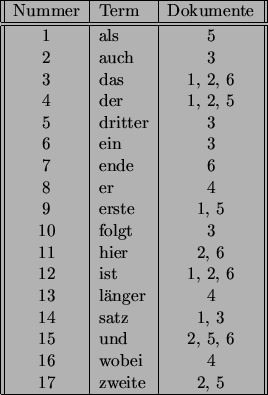
\includegraphics[scale=0.5]{../Abbildungen/index.png}
	\rule{\textwidth}{0.4pt}
	\caption{Beispiel für einen invertierten Index \cite{index_Uni_Munich}}
	\label{fig:invIndex}
\end{figure}

\section{Umsetzung eines invertierten Index}
Nachdem das Prinzip des invertierten Index klar ist, steht die Frage im Raum, wie dieser umgesetzt werden kann.
Es liegt nahe als Datenstruktur einen Trie einzusetzen. Ein Trie ist ein spezieller Suchbaum, welcher besonders gut zum Suchen von Zeichenketten geeignet ist \cite[S. 50 f.]{IR_Intro_Cambridge}.
\newline
Alternativ kann über den Einsatz einer Hashmap nachgedacht werden, jedoch führt dies zu folgendem Problem:
Angenommen die Terme einer vom Nutzer eingegebenen Query sind nicht in der Hashmap vorhanden, dann wird die Hash-Funktion keinen passenden Eintrag finden. Da in einer Hashmap Wörter, die ähnlich zueinander sind, nicht unbedingt benachbart gespeichert werden und keinerlei Information darüber bekannt ist, wo zur Query ähnliche Wörter gespeichert sind, kann im Falle, dass ein oder mehrere Wörter der Query nicht vorhanden sind, nicht mit geringem Aufwand nach ähnlichen Wörtern gesucht werden. Bei Tries besteht dieses Problem nicht \cite[S. 50]{IR_Intro_Cambridge}. 
\newline
\begin{comment}
	Da in der Beispielimplementierung ein Trie als Datenstruktur zum Einsatz kommen wird, soll diese kurz vorgestellt werden.
\end{comment}

Da die Beispiel-Implementierung, die später vorgestellt wird, jedoch möglichst einfach sein soll, wird zunächst eine Hashmap als Datenstruktur verwendet. 

\subsection{Tries}
Ein Trie wird auf der Basis einer Menge von Zeichenketten aufgebaut. Jede Zeichenkette, die gefunden werden muss, ist innerhalb des Tries repräsentiert.
\newline
Erreicht wird dies dadurch, dass ein Knoten jeweils ein Zeichen repräsentiert und eine Liste mit Verweisen auf die nächsten möglichen Knoten hält, basierend auf einem weiteren Zeichen.
Die Abbildung \ref{fig:trie} zeigt einen Trie.

\begin{figure}
	\centering
	\rule{\textwidth}{0.4pt}
	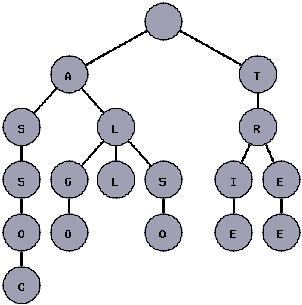
\includegraphics[scale=0.7]{../Abbildungen/trie.png}
	\rule{\textwidth}{0.4pt}
	\caption{Beispiel eines Tries \cite{trie_Abb}}
	\label{fig:trie}
\end{figure}

Im Folgenden soll eine formale Definition eines Tries gegeben werden:
\begin{defi}[Trie]\cite{Trie_wiki}
	Sei $\sum$ eine endliche Menge von Zeichen (Alphabet) und $\sum^{*}$ die Menge aller Wörter, die über $\sum$ gebildet werden können und sei $S$ $\subseteq$ $\sum^{*}$. Sei $V$ die Menge aller Knoten und $E$ die Menge aller Kanten. Jeder Knoten $v \in V$ besitzt einen Wert $w$, eine Liste $C = [c_1, .., c_n]$, wobei $c_1, .., c_n \in \sum$, und eine Liste $K = [k_1, .., k_n]$ von Knoten. Jede Kante $e \in E$ ist eine Verbindung von zwei Knoten $v_1, v_2 \in V$. Dann ist $T = (V, E)$ ist ein Trie, wenn gilt:
	
	\begin{itemize}
		\item $\forall e \in E: e$ ist mit Zeichen aus $\sum$ beschriftet.
		\item $\forall v \in V:$ alle ausgehenden Kanten von $v$ sind unterschiedlich beschriftet mit einem Zeichen $z \in \sum$
		\item $\forall S_i \in S: \exists v \in V: S_i$ ist ein Präfix der Konkatenation der Beschriftungen des Pfades vom Wurzelknoten bis $v$.
		\item $\forall b \in V: \exists S_i \in S:$ Die Konkatenation der Beschriftungen von der Wurzel bis $b$ ergibt $S_i$, sofern $b$ ein Blatt des Tries ist.
	\end{itemize}
	
\end{defi}

Das Suchen nach gespeicherten Wörtern gestaltet sich nun verhältnismäßig einfach: Um das Wort \glqq Tree\grqq\ im, in der Abbildung gezeigten, Trie zu finden, wird wie folgt vorgegangen:
\newline 
Stellt der User die Anfrage \glqq Tree\grqq, wird diese Query nun Zeichen für Zeichen durchgegangen. Beginnend bei \glqq T\grqq\ wird im Wurzelknoten geprüft, ob es einen Verweis auf einen Knoten gibt, der ein \glqq T\grqq\ repräsentiert. Existiert ein solcher Knoten, wird in diesem geprüft, ob es einen Knoten gibt, der das nächste Zeichen in der Query (das \glqq r\grqq) repräsentiert. Ist dies der Fall, wird das Verfahren solange wiederholt, bis die Query komplett eingelesen ist oder in der Query ein Zeichen steht, das durch keinen Knoten im Trie repräsentiert ist \cite{trie_Abb} \cite{Trie_Blog}.
\newline \newline
Ähnlich leicht funktioniert das Einfügen neuer Wörter in den Trie. Dazu wird - wie beim Suchen - das Wort, das eingefügt werden soll, so weit wie möglich nach dem oben beschriebenen Muster eingelesen und es wird zu den entsprechenden Knoten gesprungen \cite{Trie_Blog}. Wird nun ein Zeichen eingelesen, das nicht durch einen Knoten repräsentiert ist, wird ein neuer Knoten erzeugt, welcher dieses Zeichen repräsentiert. Alle nun noch einzulesenden Zeichen erhalten einen neuen Knoten, da der neu erzeugte Knoten natürlich nicht auf bereits vorhandene Knoten zeigen kann. Innerhalb dieses Knotens wird eine Liste angelegt, die Verweise auf weitere Knoten hält \cite{trie_Abb}. In dieser Liste wird ein Verweis auf den Knoten angelegt, der das nächste Zeichen des einzufügenden Wortes repräsentiert. Dieses Verfahren setzt sich solange fort, bis das neue Wort vollständig eingelesen ist.
\newline \newline
Das Löschen soll in diesem Rahmen nicht aufgezeigt werden, da dies weitaus komplexer sein kann als das Finden oder Einfügen von Einträgen.
\newline \newline
Ein Knoten, zu dem man mit dem Wort $S_i$ gelangt, muss außerdem eine Liste mit Verweisen auf alle Dokumente, in denen das Wort $S_i$ vorkommt, speichern. Diese Liste kann nicht leer sein, da das entsprechende Wort $S_i$ nicht im Trie vorkommen würde, sofern es in keinem Dokument steht.

\begin{comment}
\section{Komprimierung des Index}
Bei großen Dokumentenmengen wächst die Größe des Index ebenfalls. Doch nicht nur die Größe des Index wächst, sondern auch die benötigte Zeit, um auf eine Query zu antworten \cite{IR_Intro_Cambridge}.
Die Index-Komprimierung adressiert genau dieses Problem. Über die Jahre der Forschung haben sich einige Komprimierungs-Techniken bewährt und sind bei den allermeisten aktuellen Suchmaschinen in Benutzung. \newline
Dieser Abschnitt soll das Thema Komprimierung erläutern, das Hauptaugenmerk liegt dabei auf der Komprimierungs-Technik, die in der Beispielimplementierung eingesetzt wird.

\subsection{Nutzen der Komprimierung}
Bevor die technischen Details der Komprimierung betrachtet werden, sollen zunächst die Vorteile, die sich durch die Komprimierung ergeben, aufgezeigt werden.
\\
In erster Linie wird durch die Komprimierung Platz auf dem Speichermedium, auf dem der Index liegt, gespart. Liegt dieser beispielsweise in einer Datei auf einer Festplatte, zieht die Komprimierung noch weitere Vorteile mit sich: Bei Schreib- bzw. Leseoperationen auf die Datei, müssen durch die Komprimierung weniger Bytes vom Hauptspeicher zur Festplatte bzw. umgekehrt, transportiert werden. Dadurch verringert sich die I/O-Zeit \cite[S. 58, 86]{IR_Intro_Cambridge}. Weiter kann ein größerer Teil des Indexes im Cache gehalten werden, was den Zugriff auf den Index beschleunigt, da weniger I/O-Operationen auf der Festplatte erforderlich sind \cite[S. 58, 86]{IR_Intro_Cambridge}.

\subsection{Dictionary komprimieren}
In \ref{txt:inverted_index} wurde beschrieben, dass sich der invertierte Index in das Dictionary und die Posting-Listen aufteilt.
Dies sind die beiden Punkte, an denen bei der Komprimierung angesetzt werden kann.
Die erste Möglichkeit, die genauer betrachtet werden soll, ist die Dictionary-Kompression.
Der Idee, die betrachtet werden soll, liegt zugrunde, dass in der Datenstruktur, die zur Suche der Wörter, die in der Query enthalten sind, genutzt wird, in jedem Knoten ein Zeichen gespeichert wird. Wird UTF-8 zur Zeichencodierung verwendet, fällt pro Zeichen mindestens $1$ Byte an, das in jedem Knoten gespeichert werden muss. Meist besteht ein in UTF-8 codiertes Zeichen jedoch aus mehr als einem Byte. \\
Eine Möglichkeit, Speicherplatz zu sparen, ist, nicht ein Zeichen pro Knoten zu speichern, sondern lediglich einen Pointer auf ein Zeichen. Der Pointer wird als Index auf eine Liste verwendet, welche alle Zeichen enthält, die in den Dokumenten vorkommen, die der Index \glqq kennt\grqq. Ist die dem Index zugrunde liegende Datenstruktur ein B-Baum oder ein Binärbaum, kann noch weiter Speicherplatz gespart werden, indem der Liste Teilstrings hinzugefügt werden, die in mehreren Wörtern vorkommen. Da im Rahmen dieser Arbeit jedoch ein Trie verwendet wird, wird dieser Punkt nicht weiter betrachtet, da ein Trie eine solche Komprimierung bereits liefert, da jeder Substring lediglich einmal abgespeichert wird.
\\
\\
Ein Beispiel soll aufzeigen, wie mittels Pointern Speicherplatz gespart werden kann. Dazu zunächst eine Rechnung, wie viel Speicherplatz durch Zeichen in einem klassischen Trie benötigt wird:
Sei $T_1$ ein Trie mit einer Knotenzahl von $15$ Knoten. Jeder der Knoten beinhaltet ein Zeichen, welches jeweils $2$ Byte benötigt. Somit werden $15 \ * \ 2 \ = \ 30$ Byte benötigt, um alle Zeichen zu speichern. 
\\
Wird nun die Dictionary-Komprimierung angewendet, so wird eine Liste mit allen Zeichen, die in den eingelesenen Dokumenten vorkommen, angelegt. Die Größe dieser Liste bleibt beim Hinzufügen neuer Dokumente in den Index konstant, sofern die Dokumente keine bisher unbekannten Zeichen beinhalten. Die Größe der Liste ist somit für große Tries, wie sie in einem Index gewöhnlicherweise entstehen, vernachlässigbar. 
\\
Die Liste $l$ habe $26$ Einträge und beinhaltet das Alphabet von a-z ohne Umlaute.
Jeder Knoten im Trie muss jetzt lediglich einen Zeiger auf einen Listeneintrag abspeichern. Damit werden nur noch $log_2(26) \approx 4,7$ Bits benötigt. Da aufgerundet werden muss, werden 5 Bits zum Speichern des Zeigers benötigt. Damit wird eine Einsparung von $11$ Bits pro Knoten erreicht, wodurch im gesamten Trie $T_1$ $11 \ * \ 15  \ = \ 165$ Bits eingespart werden, was $20$ Bytes entspricht.
\\
Um noch weitere Zeichen in die Liste aufnehmen zu können, kann pro Zeiger ein Byte genutzt werden. Dadurch können $256$ Zeichen unterstützt werden und dennoch werden im Trie $T_1$ $15$ Bytes eingespart.
Dies wird Byte-Alignment genannt.
\\
In diesem Beispiel scheint sich der Nutzen der Komprimierung in Grenzen zu halten, betrachtet man jedoch einen Trie $T_2$ mit einer Knotenzahl von $10.000$, ergibt sich ein anderes Bild: 
Statt $10.000 \ * \ 2 = 20.000$ Byte werden mit Byte-Alignment nur noch $10.000$ Byte benötigt, wodurch $50\%$ Speicherplatz gespart werden, sofern der marginale Speicherbedarf der Liste $l$ nicht mit einbezogen wird.

\subsection{Postings-Liste komprimieren}
Weitaus mehr Speicher wird von den Posting-Listen benötigt, die im Index gespeichert werden müssen. Zur Erinnerung: Die Einträge in einer Posting-Liste verweisen auf diejenigen Dokumente, in denen das entsprechende Wort bzw. der entsprechende Term vorkommt.
\\
Der Speicherbedarf der Posting-Listen über den gesamten Index kann nicht so einfach berechnet werden wie der Speicherbedarf des Dictionarys. Im Falle eines Tries lässt sich die Anzahl der benötigten Bytes für das Dictionary mit $ Anzahl \ Knoten \ * \ Bytes \ pro \ Zeichen$ berechnen. Da die Posting-Listen jedoch unterschiedliche Längen pro Knoten aufweisen, lässt sich keine solch einfache Formel finden.
\\
Durchschnittlich benötigen Posting-Listen mehr Speicher pro Knoten als die Byteanzahl eines zu speichernden Zeichens. Werden die Dokumenten-IDs (oder Postings) mit 4-Byte-Integern abgespeichert, benötigt eine Liste $l$ $|l| \ * \ 4$ Bytes. mit 4-Byte-Integern können auf $2^{32}$ Dokumente referenziert werden, was bei großen Dokumentenmengen schnell zu Problemen führt, da weit mehr Dokumente im Index aufgenommen werden müssen. Werden 8-Byte-Integer genutzt, so können $2^{64}$ Dokumente referenziert werden, die Posting-Liste $l$ benötigt dann $|l| \ * \ 8$ Byte.
\\
Werden in der Liste statt der echten Dokumenten-ID lediglich die Differenzen zwischen den einzelnen Einträgen gespeichert, können kleinere Zahlen genutzt werden. Die folgenden zwei Tabellen zeigen, wie das aussehen könnte:


\\
Kleinere Zahlen können mit weniger Bits codiert werden, wie dies umgesetzt wird, ist Gegenstand der nächsten Abschnitte.
Es gibt mehrere Verfahren, wie diese Liste komprimiert werden kann bzw. die Integer-Werte, die in der Liste enthalten sind. Es wird dabei zwischen byte- und bit-orientierten Codes unterschieden. Im Folgenden werden zwei Varianten vorgestellt, Variable Byte Encoding und $\gamma$-Codes.

\subsubsection{Variable Byte Encoding (VBE)}
Dieser Code fällt - wie der Name bereits zeigt - in die Kategorie der byte-orientierten Komprimierung.
\\
In den meisten Computersystemen werden Integer als 4-Byte-Integer dargestellt.
Wie oben gezeigt, müssen jedoch nur noch kleine Zahlen gespeichert werden. Es wäre Verschwendung, kleine Zahlen, die mithilfe ein oder zwei Bytes codiert werden können, als 4-Byte-Integer abzuspeichern, bei dem zwei Byte lediglich führende 0en darstellen.
\\
\end{comment}